\documentclass[letterpaper]{article}

\usepackage{graphicx}
\usepackage{hyperref}
\usepackage{listings}
\usepackage{placeins}
\usepackage{float}
\usepackage[margin=1in]{geometry}

\begin{document}

% Title -----------------------------------------------------------------------

\title{CSE 40166 Final Report}
\date{12/15/17}
\author{Kyle Miller\\ {\textless}kmille42@nd.edu{\textgreater} \and Andrew Callahan\\ {\textless}acallah1@nd.edu{\textgreater} \and Christopher Clarizio\\ {\textless}cclarizi@nd.edu{\textgreater}}

\maketitle

% Overview --------------------------------------------------------------------

\section*{1. Overview}

\paragraph{}
	The original idea of our project was to create an animated simulation of a campfire. We planned to be able to choose to start and stop the fire using a button so that the simulation would show the fire would growing to its max size and then dissipating. We also planned that the fire would be textured, generate light and that the light generated by the fire would determine the lighting of the environment. Lastly, we planned to be able to move the camera around the scene using standard trackball controls.

    In order to implement our simulation we planned on using generally the same techniques that we implemented our homework assignments with. Specifically, we intended to use custom shaders and javascript code to create our simulation in the same way that we did for assignments such as the orrery. Additionally, in order to make the simulation more realistic, we intended to implement a function that would distort the flame using a system of splines and a function that would model the randomness of particles within the fire. Furthermore, we speculated that we would be able to simulate the effects of a breeze on the fire using another function that would again transform the shape of the fire.
    
    In regards to our final iteration of our project, the idea is the same (a campfire simulation) and all but one of the planned features was implemented (growth/dissipation of fire was not implemented). However, we employed a significantly different method of implementation. Instead of using WebGL and creating custom shaders for our project we used THREE.js and a library for particle simulation after its usefulness was demonstrated in class.
    

% Main Functions --------------------------------------------------------------
\section*{2. Main Functions}

\paragraph{}
    Our project was implemented almost entirely in one file, "campfire.html". Within "campfire.html", it is split into a head and a body. The head is relatively unimportant as it only sets some of the styling used. The body is where all of our simulation is done. First, we import the external scripts that we use later in our script including "three.js", "TrackBallControls.js", and "GPUParticleSysem.js".



% How to Use the Program ------------------------------------------------------
\section*{3. How to Use}

\paragraph{}
    Our project is extremely simple to use. Once you load the page the simulation will begin and you will see the campfire and the accompanying scene (i.e. logs, stones, ground and moon). You can rotate the camera by using standard trackball controls and zoom the camera in and out by using the scrollwheel on your mouse. The trackball controls, however, will not allow you to rotate beyond certain angles (i.e. it will not allow you to rotate the camera so that is below the ground). You can also adjust certain attributes of the fire such as color and size using sliders that are in a dropdown menu in the upper-right-hand corner. Lastly, you can reset and restart the simulation by clicking the button at the bottom of the dropdown menu.

% Program Results-------- ------------------------------------------------------
\section*{4. Results}

\begin{figure}[H]
\centering
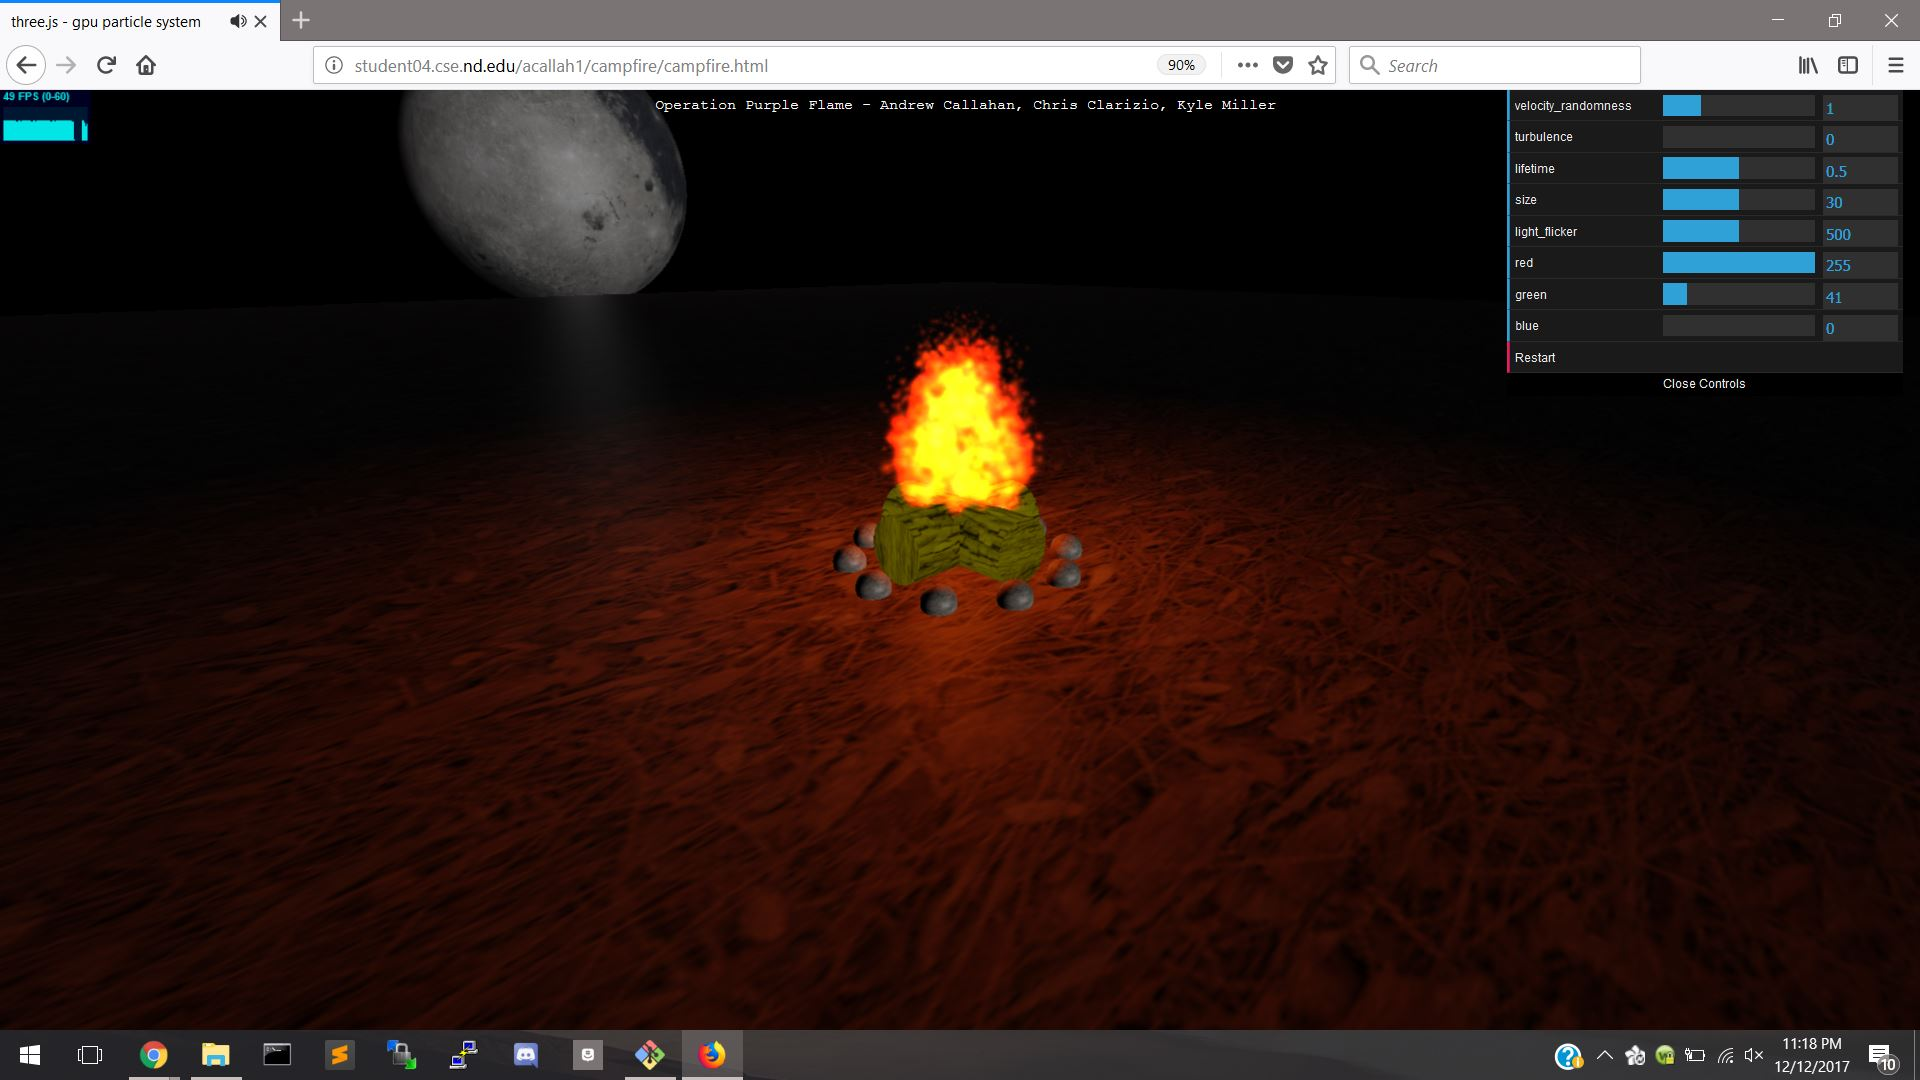
\includegraphics[scale=.35]{result1.JPG}
\caption{Basic Campfire}
\label{fig:result1}
\end{figure}

\begin{figure}[H]
\centering
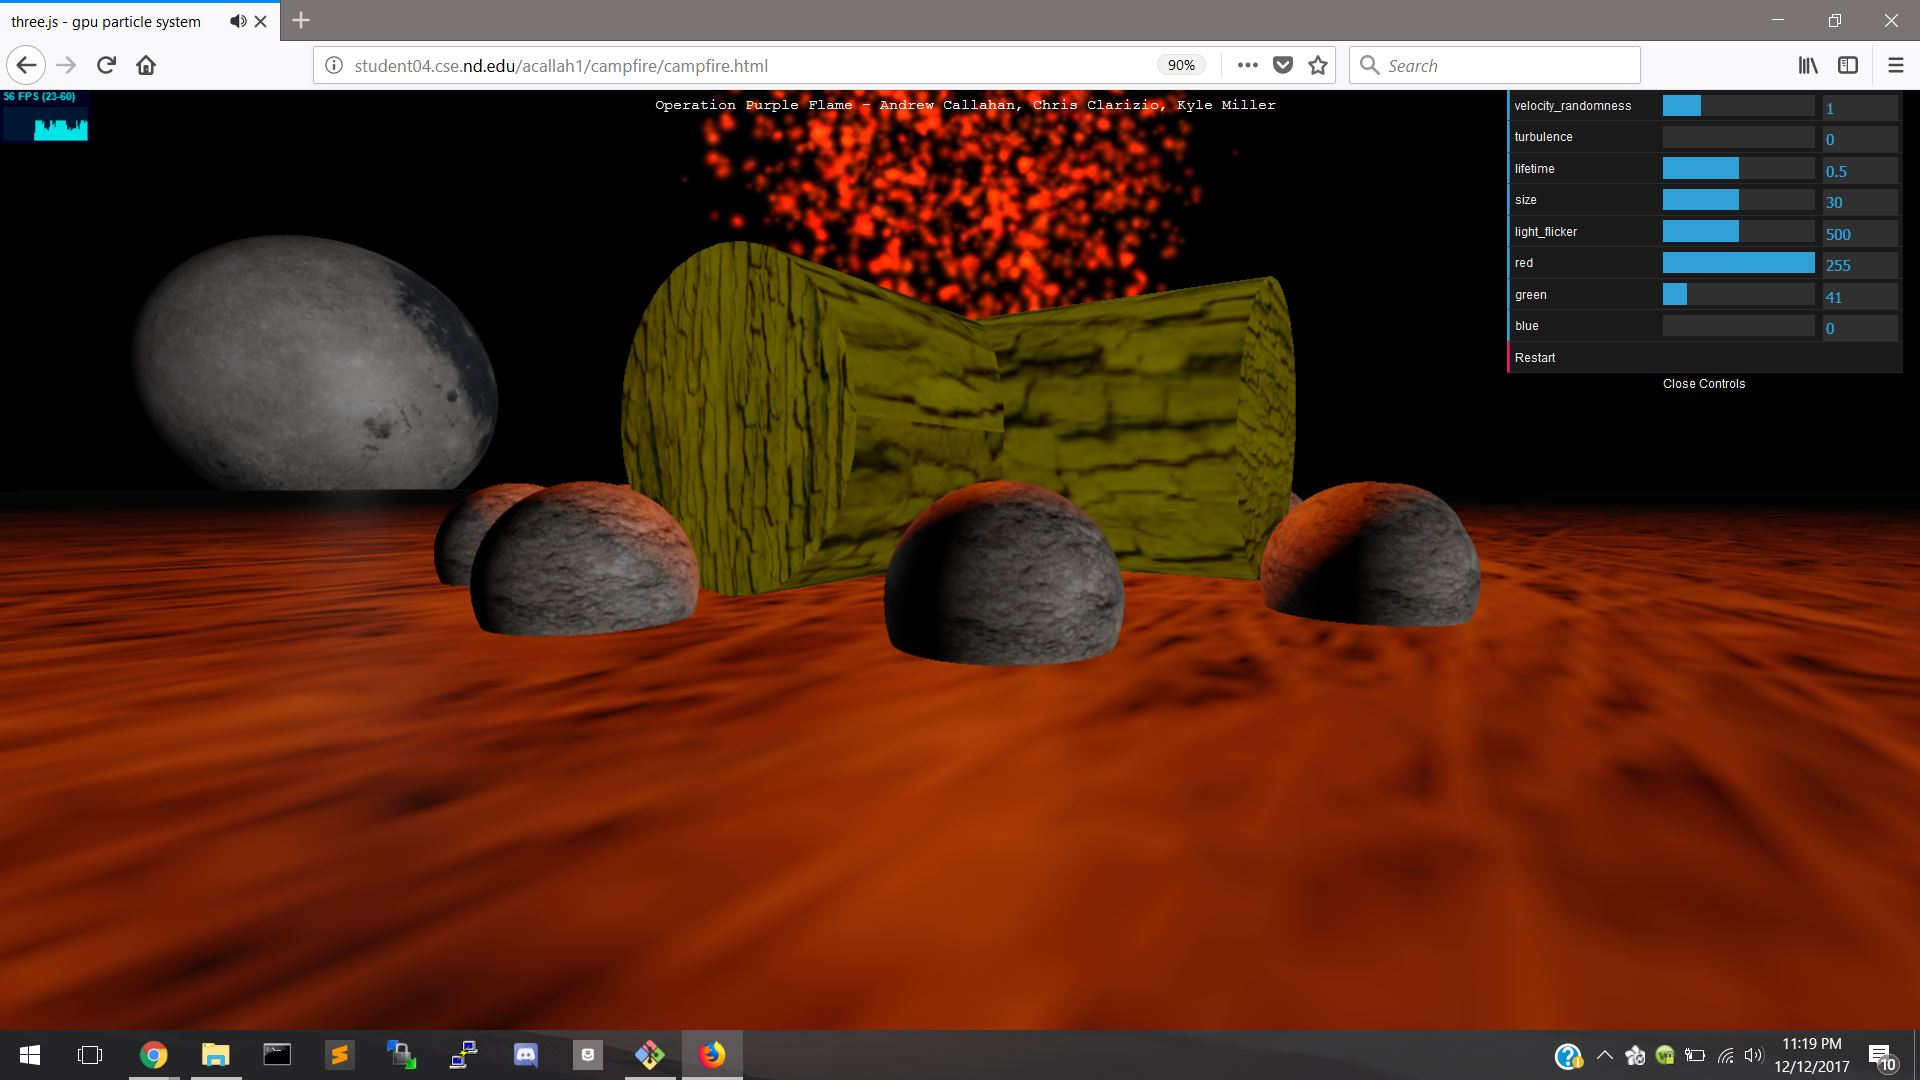
\includegraphics[scale=.35]{result2.JPG}
\caption{Moon, Rocks, Stones}
\label{fig:result2}
\end{figure}

\begin{figure}[H]
\centering
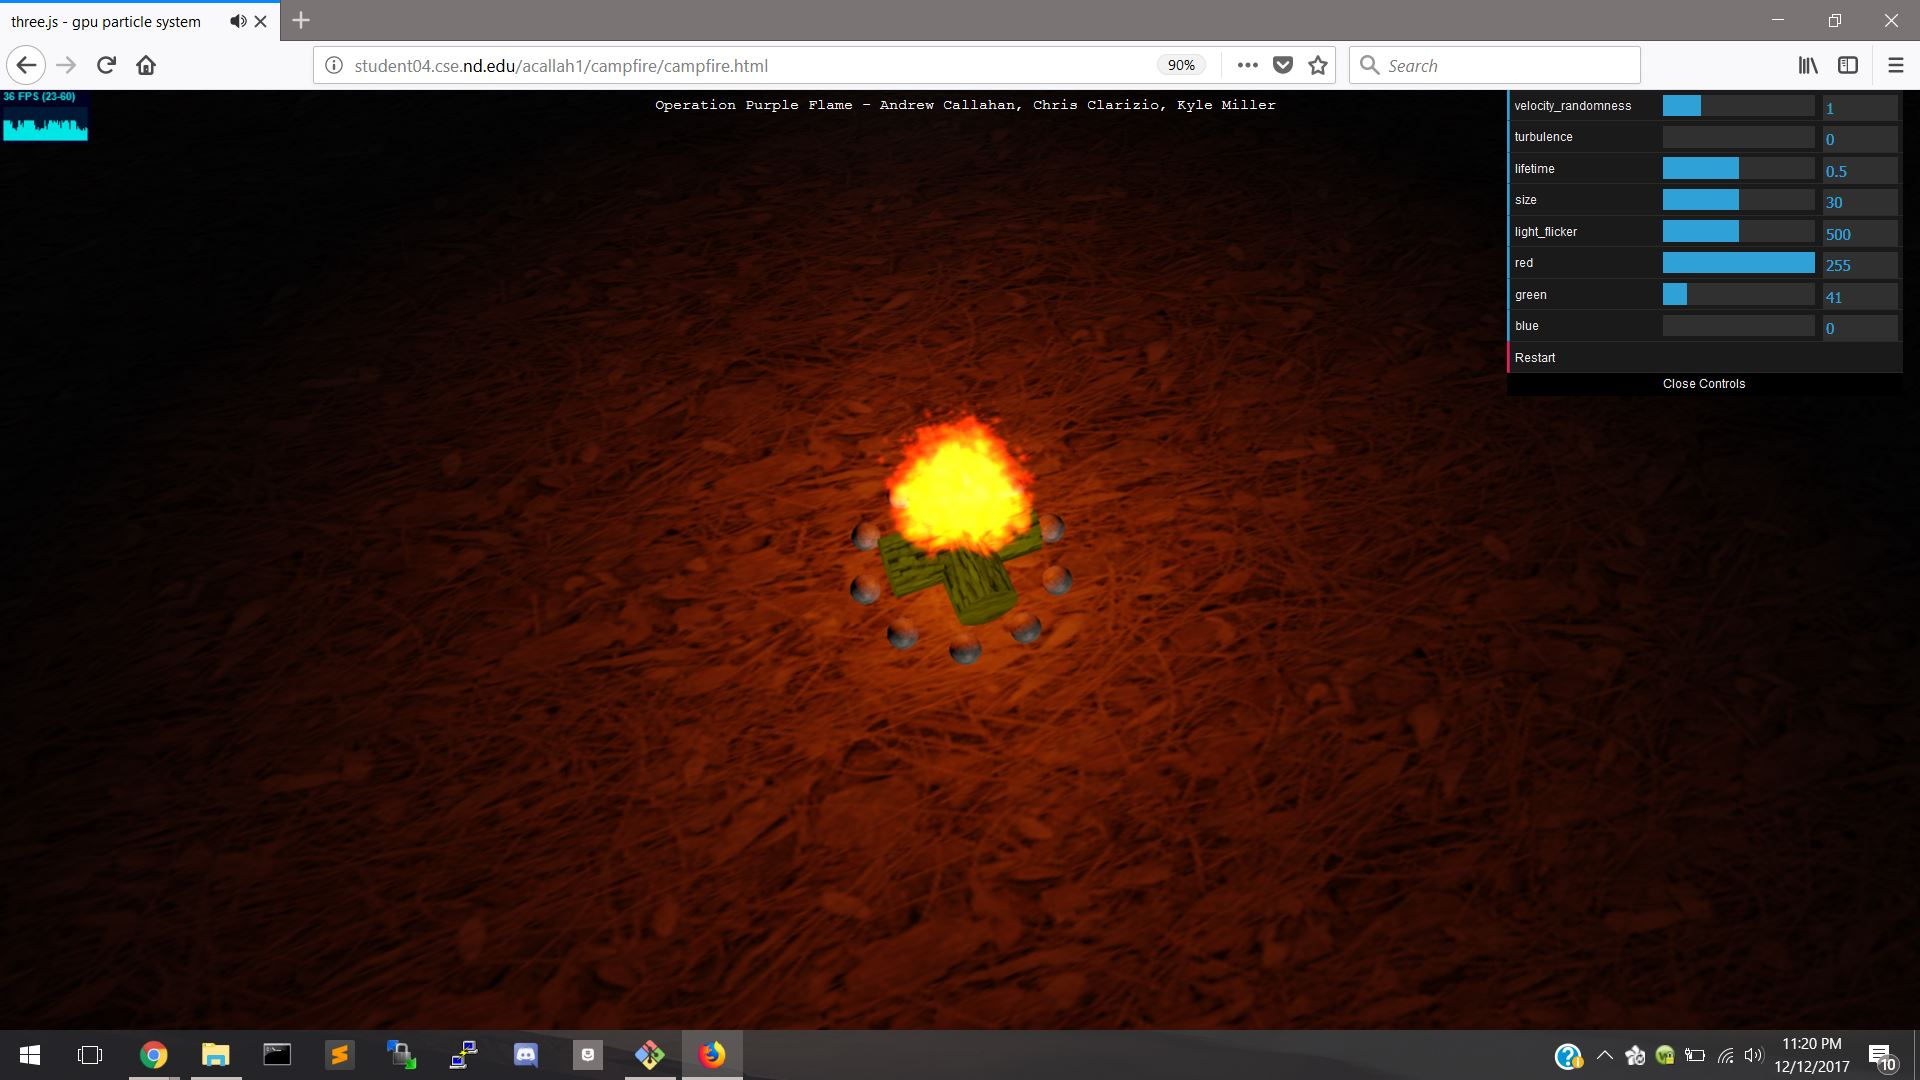
\includegraphics[scale=.35]{result3.JPG}
\caption{Ground}
\label{fig:result3}
\end{figure}

\begin{figure}[H]
\centering
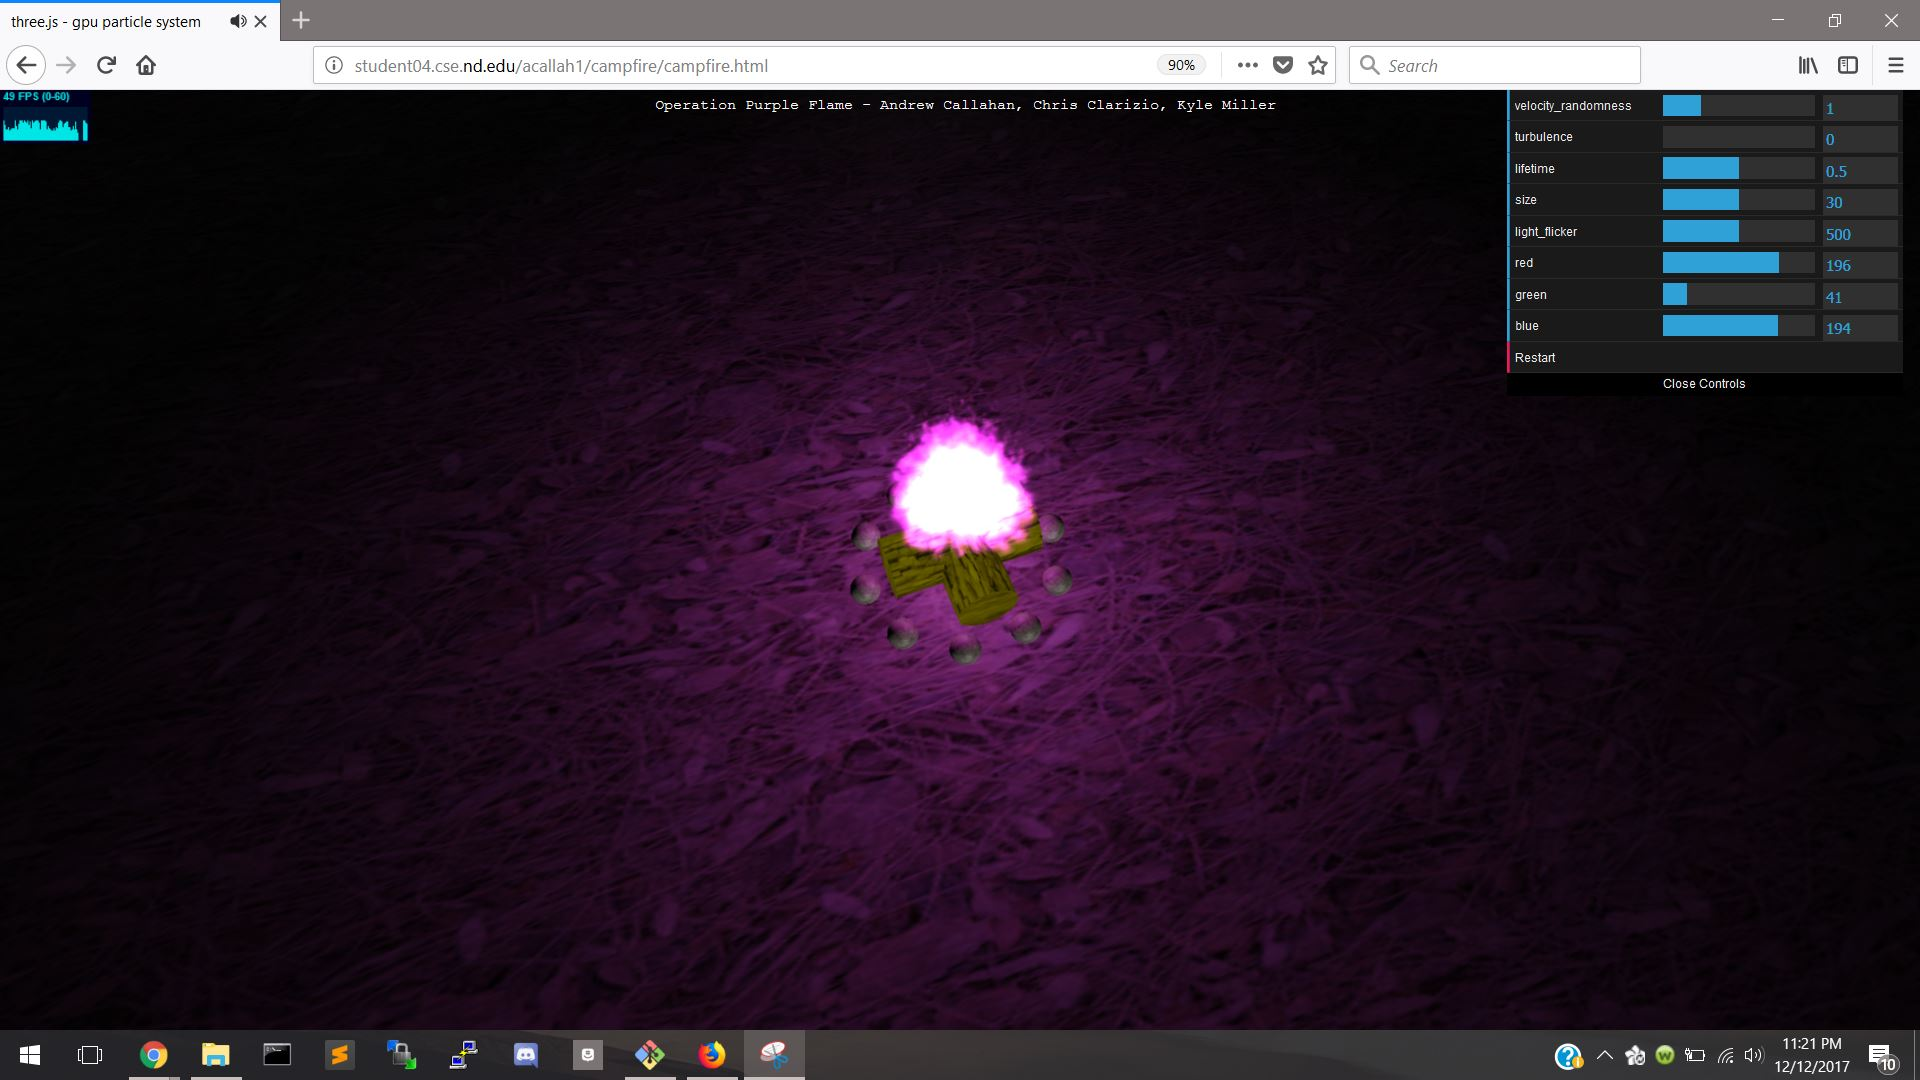
\includegraphics[scale=.35]{result4.JPG}
\caption{Colored Campfire}
\label{fig:result4}
\end{figure}

\begin{figure}[H]
\centering
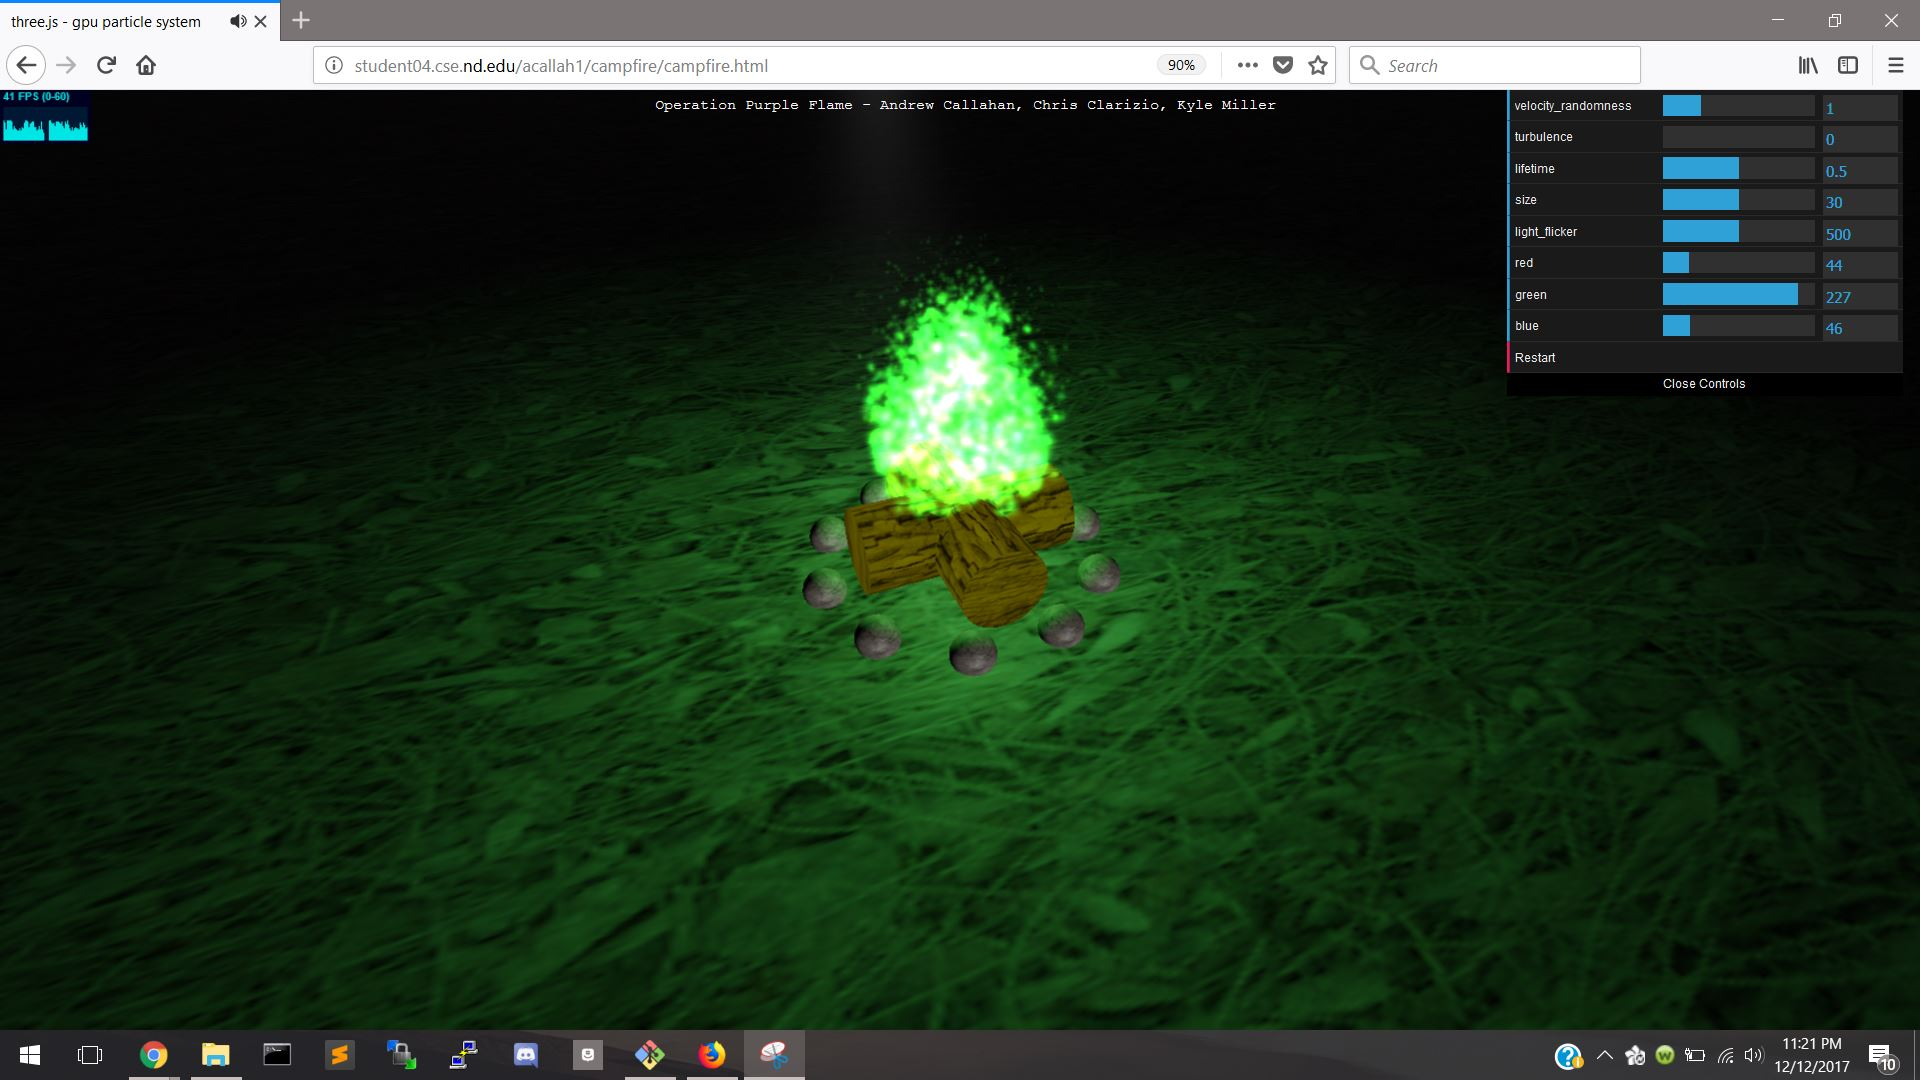
\includegraphics[scale=.35]{result5.JPG}
\caption{Colored Campfire}
\label{fig:result5}
\end{figure}

\begin{figure}[H]
\centering
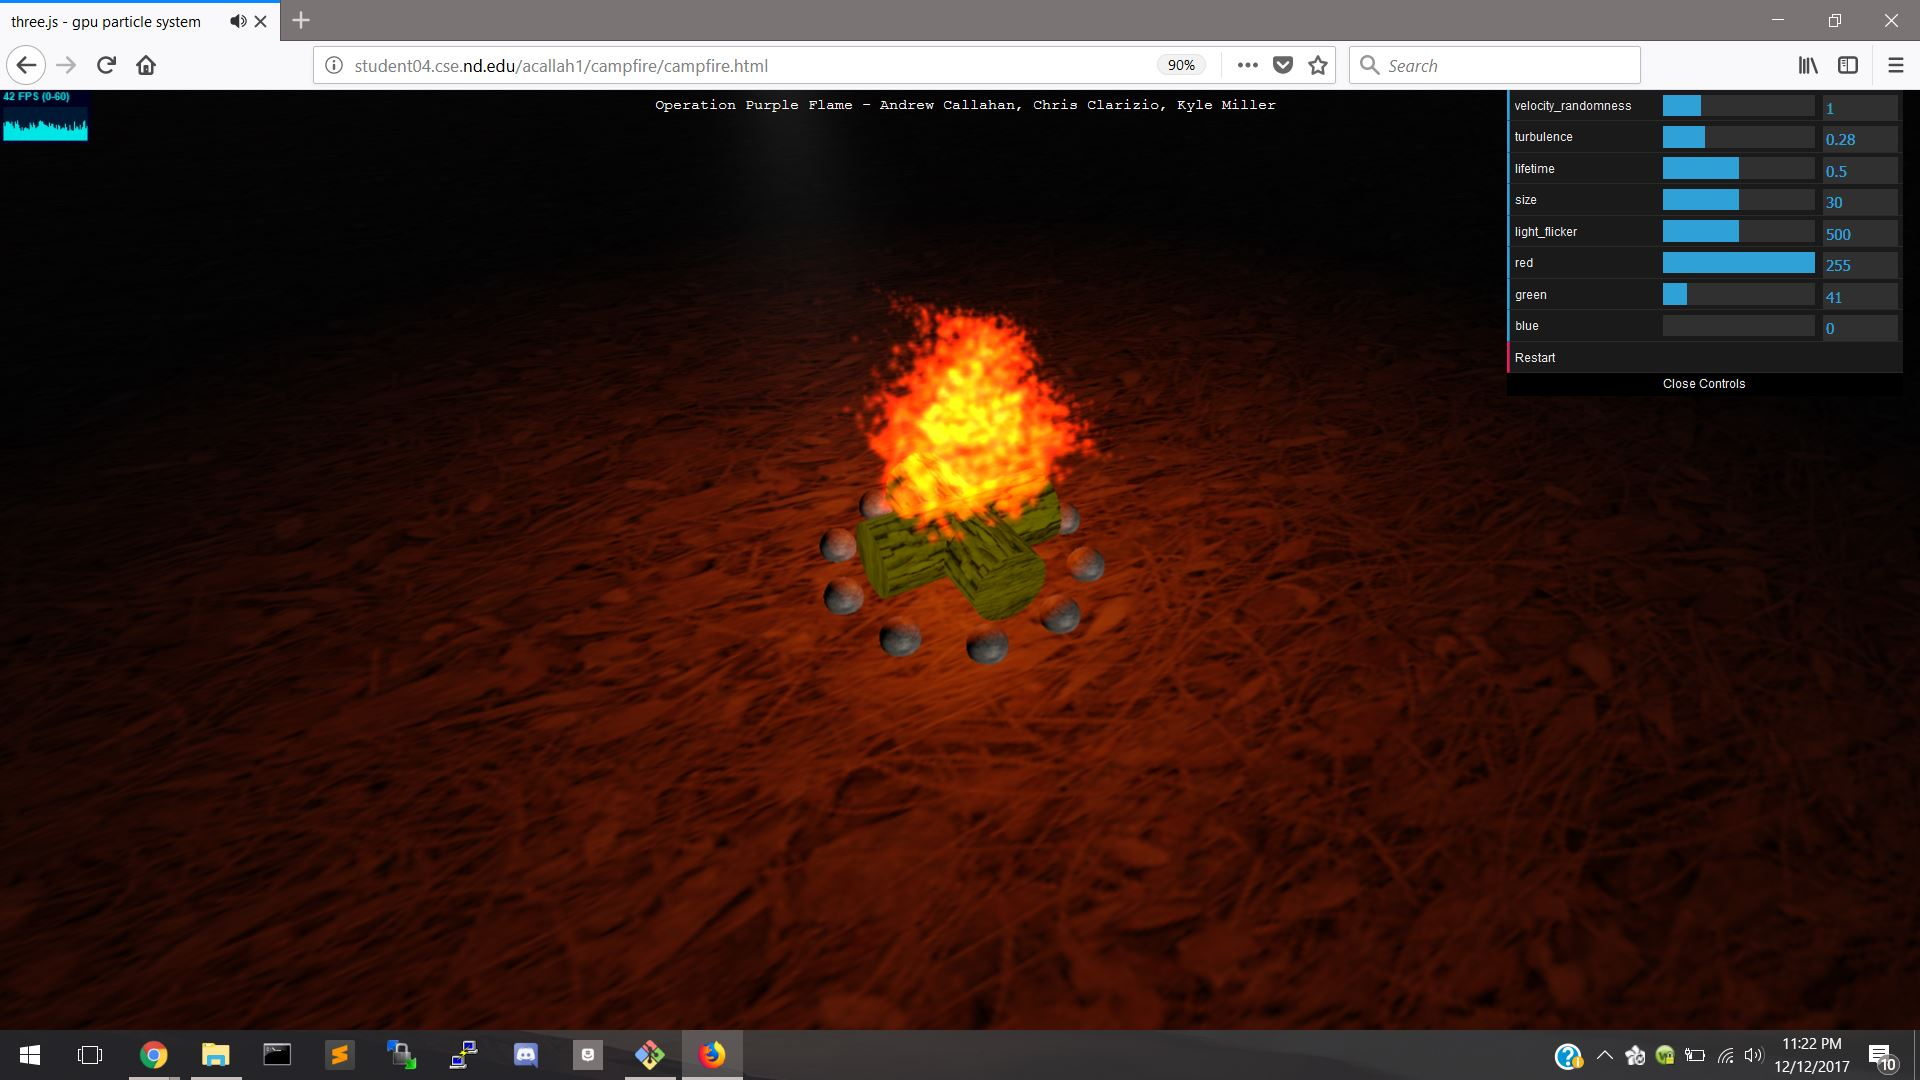
\includegraphics[scale=.35]{result6.JPG}
\caption{Turbulent Campfire}
\label{fig:result6}
\end{figure}

\begin{figure}[H]
\centering
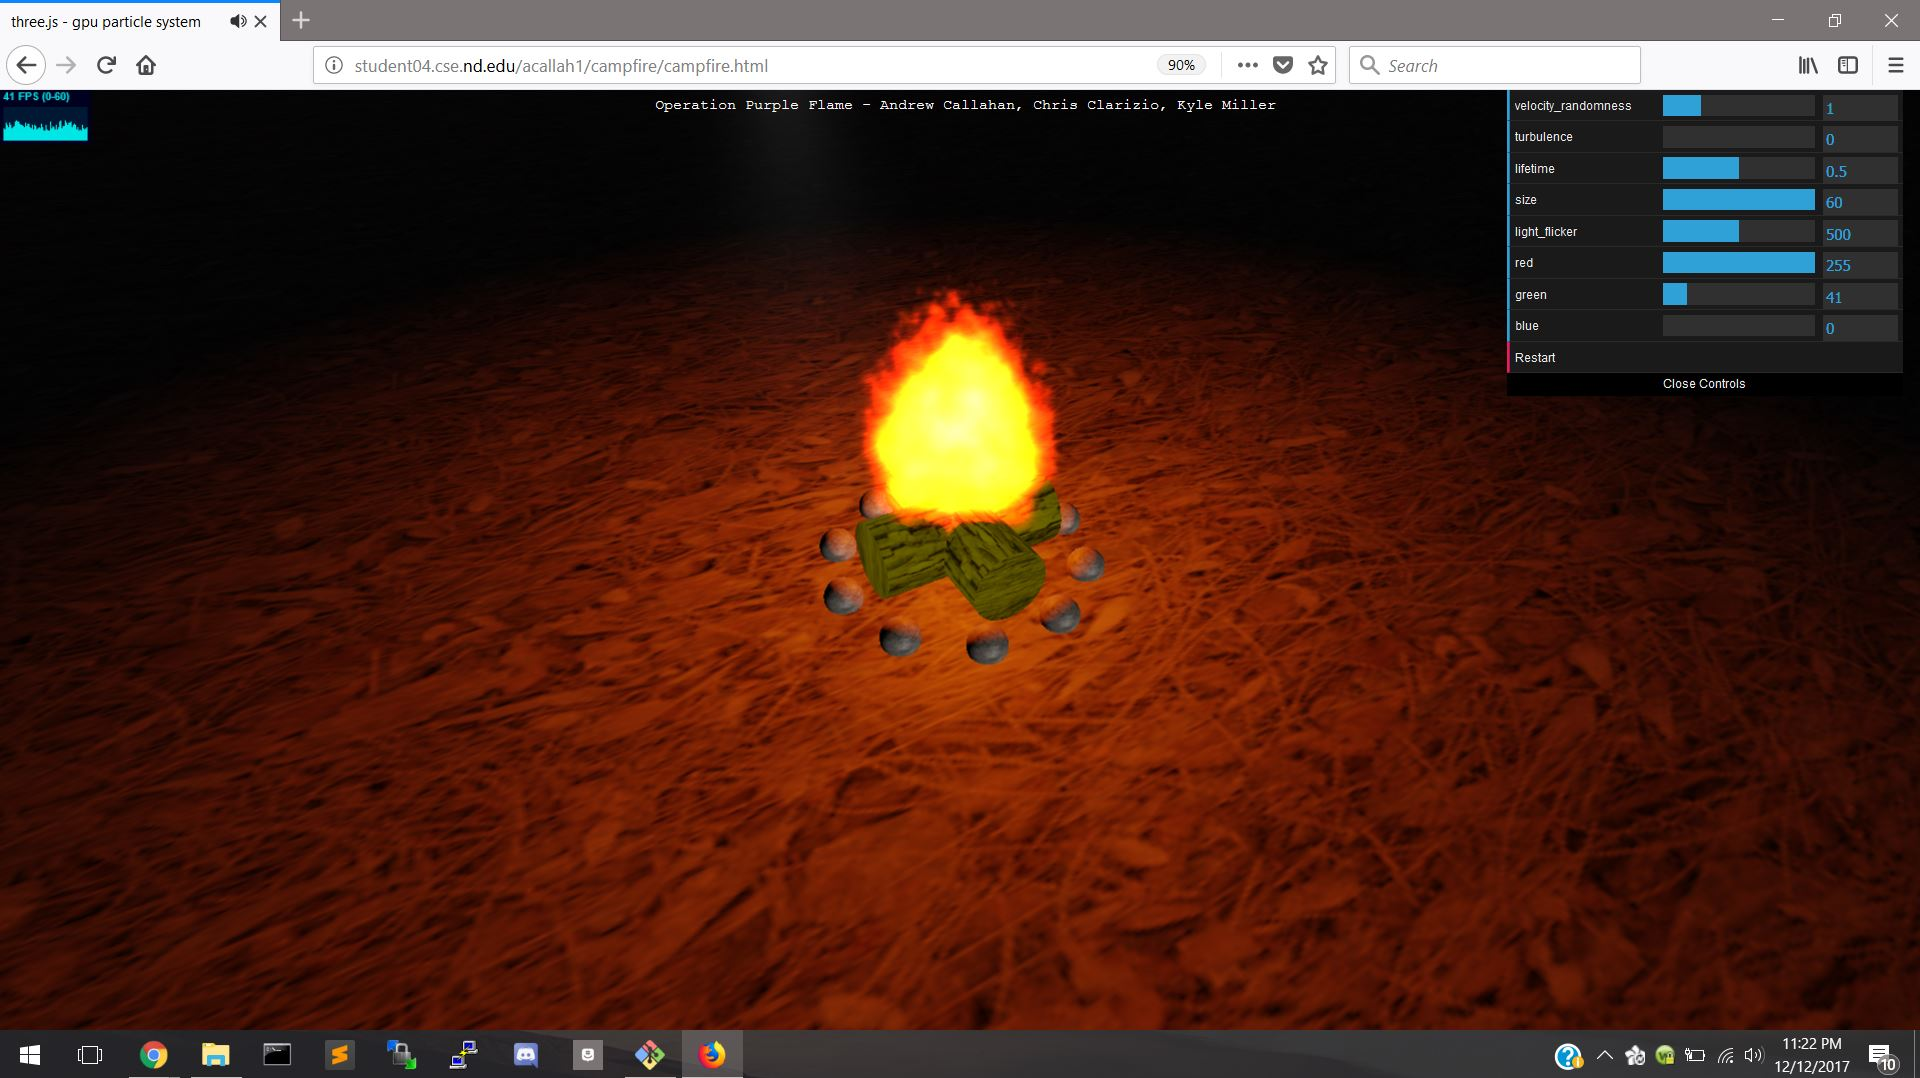
\includegraphics[scale=.35]{result7.JPG}
\caption{Campfire with Large Size}
\label{fig:result7}
\end{figure}

\begin{figure}[H]
\centering
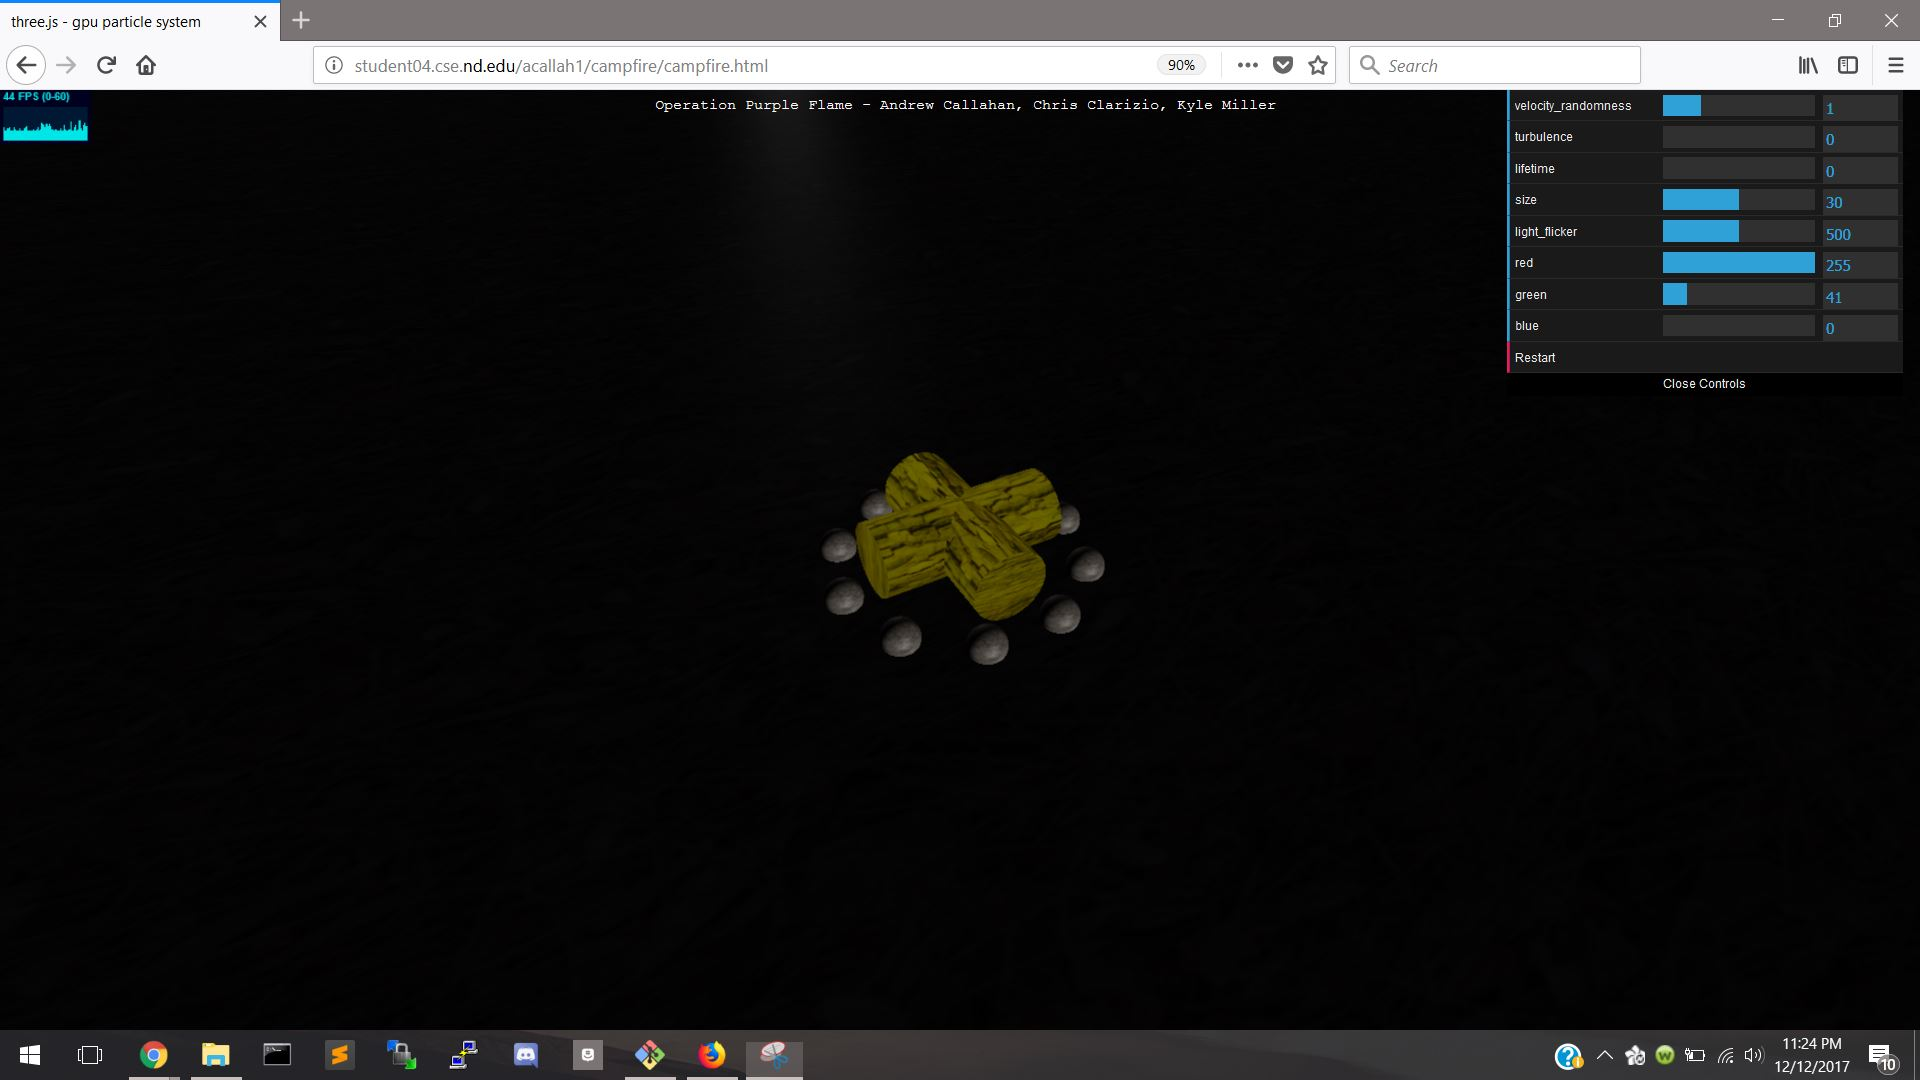
\includegraphics[scale=.35]{result8.JPG}
\caption{Campfire with Lifetime Zero}
\label{fig:result8}
\end{figure}

\begin{figure}[H]
\centering
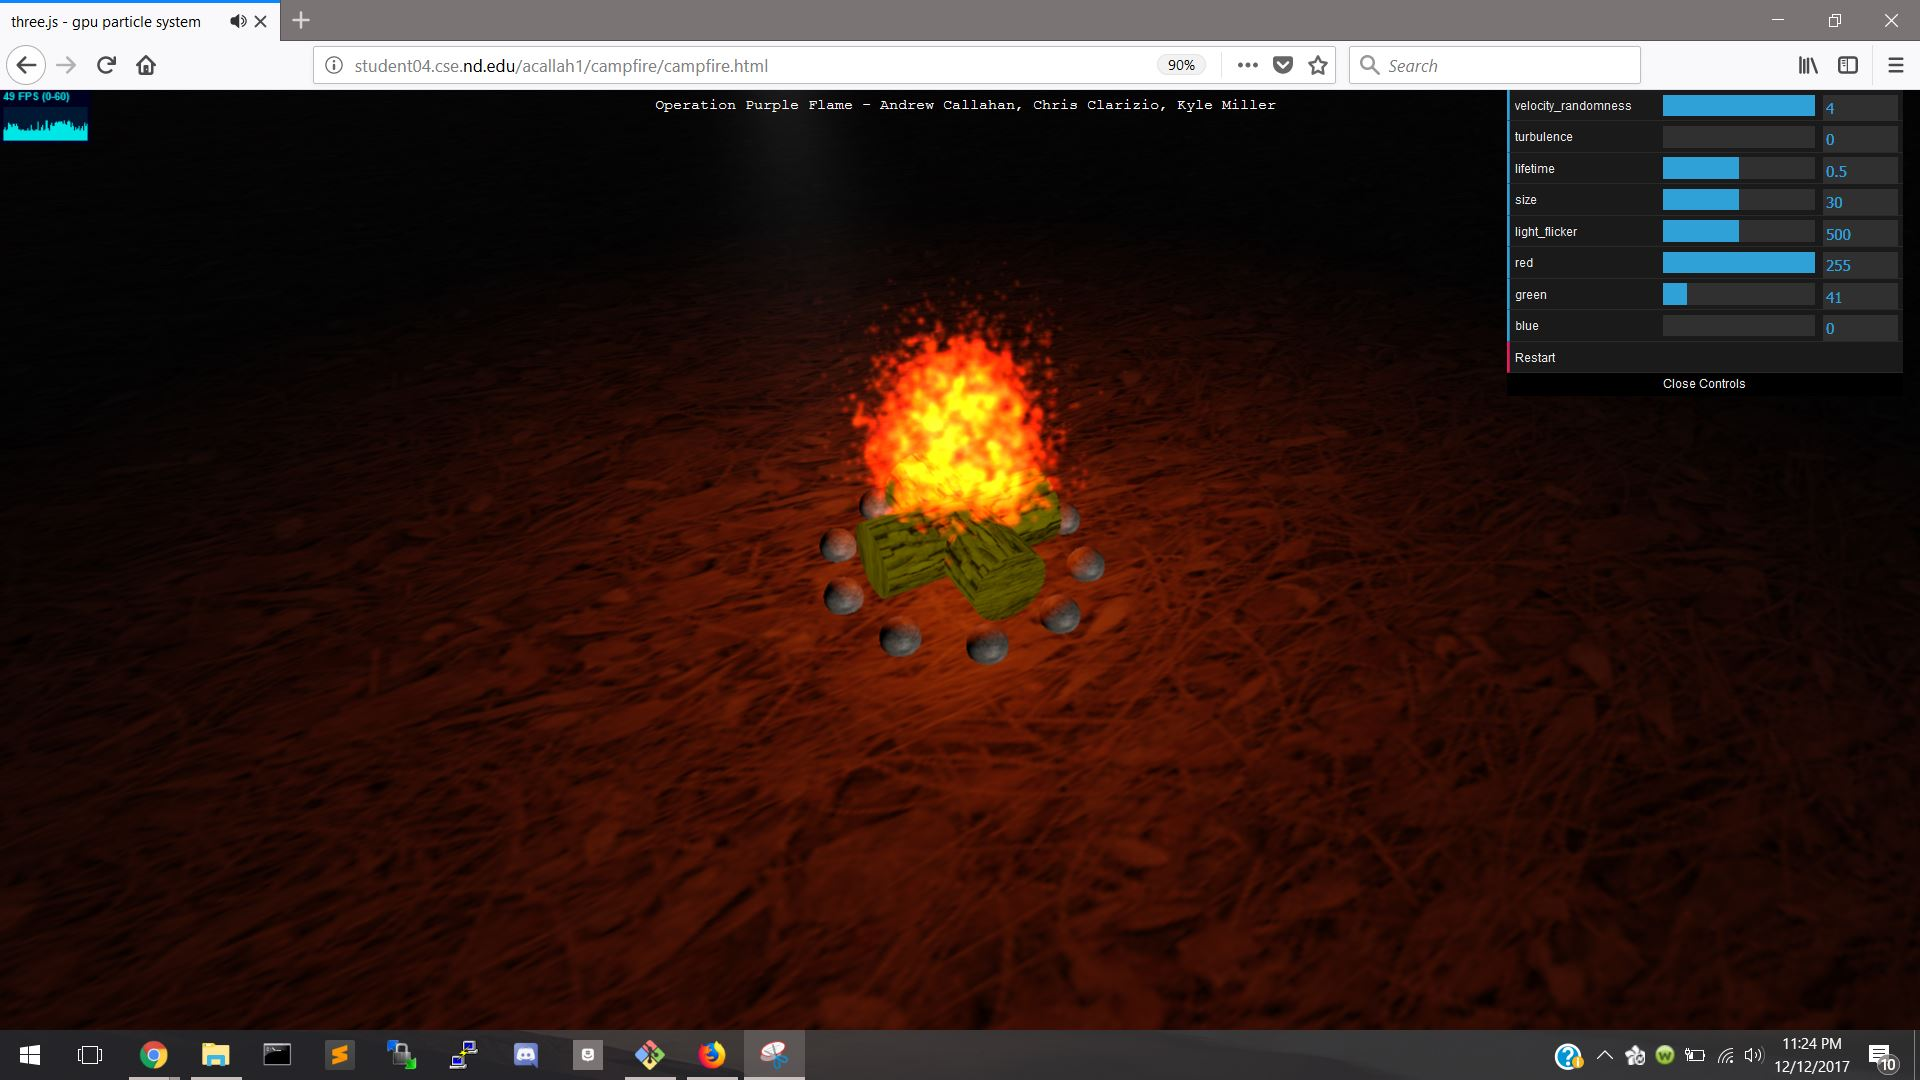
\includegraphics[scale=.35]{result9.JPG}
\caption{Campfire with Highly Random Velocities}
\label{fig:result9}
\end{figure}


% Technical Challenges -------------------------------------------------------
\section*{5. Technical Challenges}

\paragraph*{}
    filler text

% Assessement of Other Team Members ------------------------------------------
\section*{6. Assessment of Other Team Members}

\paragraph*{}
    filler text
% What I Learned -------------------------------------------------------------
\section*{7. What Was Learned}

\paragraph*{}
    filler text

\end{document}
